\section{Finite State Machine (FSM)}
\subsection{Typen}
\noindent\textbf{Mealy-System}: Wert der Ausgänge ist von Eingängen und Zuständen Abhängig. Eingänge gehen asynchron durch. Kann zu \underline{Timing Problemen} führen!

\noindent\textbf{Moore-System}: Wert der Ausgänge ist nur vom aktuellen Zustand des Systems abhängig.

\noindent\textbf{Medwedjew-System}: Spezialfall des Moore-Systems: Ausgänge entsprechen dem Zustandsvektor. \\

\subsection{Timing}
\begin{minipage}{\columnwidth}	
	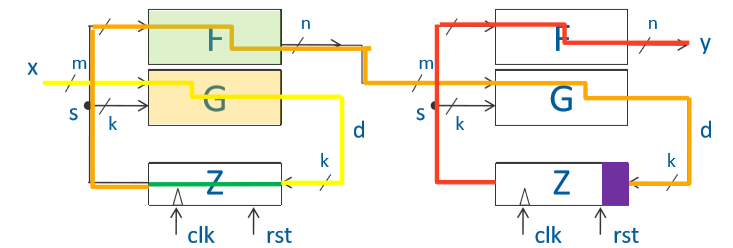
\includegraphics[width=0.8\columnwidth,keepaspectratio=true]{./Images/timingff.png}\\

	$t_{max}$ = \textcolor{green}{Propagation-Delay FF1} + \textcolor{orange}{längster Pfad von F und G Block} + \textcolor{violet}{Setup-Time FF2}. ($f \leq \frac{1}{t_{max}}$)

\end{minipage}
\\ \\
\noindent Timing von Mealy-System können nicht berechnet werden, da diese Asynchrone Anteil haben.